\documentclass[12pt]{article}

\usepackage[dvips,letterpaper,margin=0.75in,bottom=0.75in]{geometry}
\usepackage{cite}
\usepackage{slashed}
\usepackage{graphicx}
\usepackage{amsmath}
\usepackage{braket}
\usepackage{latexsym,amssymb,amsmath}
\usepackage{pdfpages}
\usepackage{xcolor}

\usepackage[american,fulldiode]{circuitikz}
\tikzset{component/.style={draw,thick,circle,fill=white,minimum size =0.75cm,inner sep=0pt}}

\begin{document}
\ctikzset{bipoles/thickness=1}
\ctikzset{bipoles/length=.6cm}

\title{Proposal for Revising the \\ Undergraduate Physics Curriculum \\ Version 1.1}
\author{Undergraduate Curriculum Committee}

\maketitle

\section{Objectives}

\begin{table}
\caption{Typical schedule for undergraduate physics majors, taking the 9H series, in the fall quarter, omitting lab courses.  Typical math courses shown in italics, but note that taking MAT 21A in fall is also common with instructor permission, with 21D taken over the summer to catch up in time for 9HD.}

\label{tbl:current-honors}
\begin{center}
\begin{tabular}{|l|l|l|l|}
\hline
year      & fall    & winter & spring  \\
\hline
Freshman  & 9HA(5)     & 9HB(5)     & 9HC(5) \\
          & {\it 21B(4)}  & {\it 21C(4)}  & {\it 21D(4)} \\
\hline
Sophomore & 9HD(5)     & 9HE(5)     & 40(4)     \\
          & {\it 22A(3)}     & {\it 22B(3)} & \\
\hline
Junior    & 104A(4) & 105B(4) & 110B(4)\\
          & 105A(4) & 110A(4) & 115A(4)\\
          & 102(1)  &      &     \\
\hline
Senior    & 115B(4) &        & \\
          & 110C(4) &        & \\
          & 112(4)  &        & \\

\hline 
\end{tabular}
\end{center}
\end{table}

\begin{table}
\caption{Typical schedule for undergraduate physics majors that transfer to UC Davis in their Junior year, omitting lab courses.}
\label{tbl:current-transfers}
\begin{center}
\begin{tabular}{|l|l|l|l|}
\hline
year      & fall    & winter & spring  \\
\hline
Junior    & 9D(4)   &         & 40(4)   \\
          & 104A(4) & 105B(4) & 110B(4) \\
          & 105A(4) & 110A(4) & 115A(4) \\
          & 102(1)  &       & \\
\hline
Senior    & 110C(4) &        & \\
          & 115B(4) &        & \\
          & 112(4)  &        & \\
\hline 
\end{tabular}
\end{center}
\end{table}

The current typical schedule of student coursework is shown in Table~\ref{tbl:current-honors} for students taking Honor's physics.  The schedule for transfer students that arrive at UC Davis for their Junior year is shown in Table~\ref{tbl:current-transfers}.  There are many different trajectories through our program, but most are some variation on these two.  This proposal aims to improve upon this course of study, to achieve the following aims:
\begin{itemize}

\item Physics majors that complete 9HD or 9D in the fall of their sophomore year have little to do for the rest of the year.  The honors students have 9HE, but this is effectively an elective and does little to further prepare them for upper division coursework.  The recent addition of 40 and 80 is helpful in that it provides something for students to do during this time, but the problem still remains that they do make progress on the upper division core coursework.  The result of this stalling is that the junior and senior year are a race to complete the degree requirements, leaving very little flexibility or time for advanced electives.

\item Transfer students that arrive at UC Davis for their Junior year face a wall of coursework that they have to handle in the first quarter: math methods, mechanics, and modern physics.  Many also take Physics 102, which is nominally a one credit course, but generally nearly as much work as a four credit course.  For many of the transfer students these courses are the first physics courses that require solving challenging homework problems, and they face effectively 16 credits.  We have two trains of students running through our program and the fall of their junior year is the train wreck where they collide.

\item The current curriculum does not include sufficient computing practice for our students.  It is useful to consider what a physics degree would like if we taught calculus the same way we teach computing.  Students would arrive their Freshman year and take an introductory calculus course.  Then, they would take their physics courses, which would never mention calculus.  At some point in their Junior or Senior year, they would take a one quarter course called ``Calculus in Physics'' which would attempt to show all the ways we use calculus in physics.  Our students are experts at calculus because they learn how to use the tool, and then apply it, again and again, throughout their coursework.  To remain relevant in the modern world (or even the world from 20 years ago) our majors need more practice in the use of computing as an essential tool for solving physics problems.

\item Within the College of Letters and Science, we are allowed to require a maximum of 110 credits in our majors, which is one half the maximum number of credits students are allowed to take.  Fitting the canon of undergraduate physics into such a tight space is extremely challenging.  Students complain that we waste time teaching some topics again and again (e.g. Special Relativity from scratch) while completely dropping other topics (e.g. Classical Hamiltonians).  The problem is particularly acute for Applied Physics majors, where core material must be dropped to make space for coursework outside of Physics.

\item The prerequisite structure of the upper division courses creates many tiers.  
As an extreme example, 122 requires 112, which requires 115A, which requires 104A and 105A, both of which require the 9 series.  This, combined with the rapid pace, leaves very little flexibility for students once they start their Junior year.  For example, missing a single quarter of the courses in the Junior year of Table~\ref{tbl:current-honors} requires an exception to prerequisites or an extra year to graduate.

\label{tbl:current-honors}

\end{itemize}

This proposal aims to make significant improvements on each of these issues.
\newpage

\section{Proposed B.S. Requirements}

The proposed B.S. Requirements are presented in Tables~\ref{tbl:prep} and \ref{tbl:core}.  Example schedules are presented in Tables~\ref{tbl:proposed-honors}-\ref{tbl:proposed-transfers}.

\begin{table}
\caption{\label{tbl:prep}Preparatory Subject Matter}
\noindent
\vskip 0.25cm
Credits:  49-50. *: recommended, C: concurrently.\\
\begin{tabular}{|llllll|}
\hline
Course & & Credits & Offered & Pre-reqs & Name \\
\hline
MAT & 21A & 4 & FWS & & Differential Calculus\\ 
    & 21B & 4 & FWS & 21A & Integral Calculus \\ 
    & 21C & 4 & FWS & 21B & Partial Derivatives and Series\\ 
    & 21D & 4 & FWS & 21C & Vector Analysis\\ 
    & 22A & 3 & FWS & 21C & Linear Algebra\\ 
    & 22B & 3 & FWS & 22A & Differential Equations\\ 
\hline
\hline
PHY & 9A & 5 & FS & 21B & Classical Physics {\it (Class. Mech.)}\\ 
    & 9B & 5 & FW & 9A,21C & Classical Physics {\it (Waves, Thermo., Optics.)}\\ 
    & 9C & 5 & WS & 9B,21D & Classical Physics {\it (Elec. and Magn.)}\\ 
    & 9D & 4 & FS & 9C,22A & Modern Physics {\it (Rel. and Quant. Mech.)}\\ 
\hline
&or&&\\
\hline
PHY & 9HA & 5 & F & C:21B/21M & Honors Physics {\it (Class. Mech.)}\\ 
    & 9HB & 5 & W & 21B/21M & Honors Physics {\it (Rel. and Stat. Mech.)}\\ 
    & 9HC & 5 & S & 21C & Honors Physics {\it (Waves and Quant. Mech.)}\\ 
    & 9HD & 5 & F & 21D & Honors Physics {\it (Elec. and Magn.)}\\ 
\hline
\hline
PHY & 40  & 4 & F & & Introduction to Physics Computation \\ 
    & 80  & 4 & FS & 40,9D & Experimental Techniques \\ 
PHY & 185* & 1 & S & & \\ 
    & 190* & 1 & F & & \\ 
\hline
\end{tabular}
\end{table}

\begin{table}
\caption{\label{tbl:core}Core Subject Matter}
\noindent
\vskip 0.25cm
Credits:  46-50. *: recommended, C: concurrently.\\
\begin{tabular}{|llllll|}
\hline
Course & & Credits & Offered & Pre-reqs & Name \\
\hline
PHY & 102  & 4 & W & 40, 9D/9HD     & Computational Physics\\
    & 104A & 4 & F & 9D/9HD, MTH 22B & Mathematical Physics \\ 
    & 105A & 4 & W & 9D/9HD, C:MAT 22B   & Classical Mechanics I\\
    & 105B & 4 & S & 105A, 102      & Classical Mechanics II\\ 
    & 110A & 4 & W & 104A, 9D/9HD   & Electricity and Magnetism I\\
    & 110B & 4 & S & 110A           & Electricity and Magnetism II\\
    & 115A & 4 & F & 104A, 9D/9HD   & Quantum Mechanics I \\
    & 115B & 4 & W & 115A           & Quantum Mechanics II \\
    & 115C & 4 & S & 115B, 102      & Applications of Quantum Mechanics\\ 
    & 112  & 4 & F & 104A, 9D/9HD   & Thermodynamics and Statistical Mechanics\\    
\hline
PHY & 116A & 4 &  F & 80   & Instrumentation with Discrete Electronics  \\
    & 116B & 4 &  W & 80   & Instrumentation with Integrated Electronics\\ 
\hline
    & or & & & & \\
\hline
PHY & 122A or B & 4 & WS & 80 & Advanced Physics Laboratory \\  
\hline
 & Any two of & & & & (all three recommended): \\
\hline 
PHY & 110L & 1 & S & 102,C:110B & Computational Lab in Electricity and Magn. \\
    & 112L & 1 & F & 102,C:112  & Computational Lab in Statistical Mechanics \\ 
    & 115L & 1 & W & 102,C:115B & Computational Lab in Quantum Mechanics \\ 
\hline
\end{tabular}\\ \vskip 0.25cm
\noindent
{\bf Electives:} an additional 15 credits of electives is required, 12 credits from advanced (capstone) topics.\\
\noindent
{\bf Total Units:} 110-115
\end{table}

\begin{table}
\caption{Example schedule for undergraduate physics majors taking the 9H series and opting for the 116 lab sequence.  X are elective courses.  Rate is 5-12 physics credits per quarter.}
\label{tbl:proposed-honors}
\begin{center}
\begin{tabular}{|l|l|l|l|}
\hline
year      & fall    & winter & spring \\
\hline
Freshman  & 9HA(5)       & 9HB(5)        & 9HC(5) \\
          & {\it 21B(4)} & {\it 21C(4)}  & {\it 21D(4)}\\
          &              &               & \\
\hline
Sophomore & 9HD(5)       & 105A(4)      & 105B(4) \\
          & {\it 22A(3)} & {\it 22B(3)} & 104A(4) \\
          & 40(4)        & 102(4)       & 80(4)  \\
\hline
Junior    & 115A(4) & 115B(4)  & 115C(4)\\
          & 112(4)  & 110A(4)  & 110B(4)\\
		  & 112L(1) & 115L(1)  & 110L(1)\\
\hline
Senior    & X(3)    & XA(4)  & 122A(4) \\
          &         & XA(4)  & XB(4) \\

\hline  
\end{tabular}
\end{center}
\end{table}

\begin{table}
\caption{Example schedule for undergraduate physics majors taking 9A in the fall of their  freshman year opting for 122A.  E is an elective course.  Rate is 0-13 physics credits per quarter.}
\label{tbl:proposed-nonhonors}
\begin{center}
\begin{tabular}{|l|l|l|l|}
\hline
year      & fall    & winter & spring \\
\hline
Freshman  & {\it 21A(4)}  & {\it 21B(4)}  & {\it 21C(4)}\\
          &               &               & 9A(5) \\
\hline
Sophomore & {\it 21D(4)}  & {\it 22A(3)}  & {\it 22B(3)}\\ 
          & 9B(5)         & 9C(5)         & 9D(4) \\
          & 40(4)         &             & 80 \\
\hline
Junior   & 104A(4)   & 105A(4)       & 105B(4) \\
         & X(3)      & 110A(4)       & 110B(4) \\         
         &           & 102(4)        & 110L(1) \\

\hline
Senior   & 115A(4)   & 115B(4)       & 115C(4) \\
         & 112(4)    & 115L(1)       & 122A(4) \\
         & 112L(1)   & XA(4)         & XB(4)  \\
		 &           & XA(4)         & \\
\hline  
\end{tabular}
\end{center}
\end{table}

\begin{table}

\caption{Example schedule for for an undergraduate physics majors that transfered to UC Davis in their Junior year without Physics D or 40 equivalents.  Rate is 12-13 credits per quarter.}
\label{tbl:proposed-transfers}
\begin{center}
\begin{tabular}{|l|l|l|l|}
\hline
year      & fall    & winter & spring \\
\hline
Junior   & 9D(4)     & 105A(4)       & 105B(4) \\
         & 40(4)     & 110A(4)       & 110B(4) \\         
         & 104A(4)   & 102(4)        & 80(4) \\
         &           &               & 110L(1) \\
\hline
Senior   & 115A(4)   & 115B(4)       & 115C(4) \\
         & 112(4)    & 115L(1)       & 122A(4) \\
         & 112L(1)   & XA(4)         & XB(4)  \\
		 & X(3)      & XA(4)         & \\
\hline 
\end{tabular}
\end{center}
\end{table}

A primary feature of this proposal is that incoming transfer students now overlap in some courses with sophomore's that took the Honor's physics sequence.  This eliminates the stalling of our honors students while relieving some of the intense academic pressure on incoming transfer students.  Our experience has been that the best of the transfer students perform as well as our four-year students once they have sufficient time to adjust, and this proposal gives them that time.  Accelerating student's that took the Honor's sequence also provides tremendous additional flexibility to their schedule.  

Transfer students that wish to complete their degree in two-years are still highly constrained, but instead of facing what amounts to 12 credits of upper division coursework upon arrival that start with four credits.  Take the time to compare fall quarter of the junior year in Tables~\ref{tbl:current-transfers} and \ref{tbl:proposed-transfers}, this is a major feature of this proposal.  This gentle introduction does not come at the cost of increased credit loads later on: transfer students can complete the degree without exceeding 13 credits of physics coursework in any quarter.  

Several new classes have been added, others require changes to their content or will no longer be required:
\begin{itemize}
\item 9A-D and 9HA-D are largely unchanged, however, some fine adjustments may be needed to ensure that the 9 series plus 104A are sufficient preparation for 112.  Also, there are some minor adjustments to the math pre-requisites.

\item 9HE is no longer offered.  This course is effectively an elective, with content that varies from instructor to instructor.  By removing it, we allow the students in the Honor's sequence to start toward the core material sooner, leaving more time for advanced electives. With more relaxed schedule in their senior year, it seems highly plausible that physics majors will take more advanced electives.

\item 102:  This new four-credit course will be renamed ``Computational Physics'' and 
will have the 9 series and 40 as prerequisites.  The focus will be on solving physics problems at the conceptual level of the 9 series using computational physics.  This course will play an integral role in this revised curriculum and so the content and tools will need to be more consistently covered than in 104B.  The decision to use 102 as the course number is for clarity, as 104A will not be a prerequisite.

\item 104A:  This course will now be offered in both Fall and Spring, as discussed further in the pre-requisites discussion.  This proposal is overall instructor revenue neutral due to the removal of 9HE.  In addition to removing the bottleneck, most students taking Honor's Physics will take the course in the spring, while most transfer students will take the course in the fall.  This will allow the course to be pitched slightly differently in these two quarters, to better reflect student preparation.

\item 105:  The timing of the 105AB sequence is adjusted to start in winter, and the content of 105A should be adjusted to include all pre-requisite material for 115A (notably  Hamiltonian mechanics).  The content of 105AB should be at a level appropriate for a sophomore completing 9HD in Fall.  There is no pre-requisite for 104A, but typically students will take 104A concurrently with 105B or before 105A.

\item 110:  The three quarter 110ABC sequence is reduced to a two course sequence 110AB, so the vector potential and special relativity will now be covered in 110B.

\item 112:  The 115A pre-requisite for 112 has been removed, and the treatment must rely on quantum from the 9 series instead.

\item The 115 sequence will be extended to a three quarter sequence 115ABC, but applied physics majors will not be required to take 115C.  The prerequisites are 104A and 105A.
The last quarter, 115C, adds 102 as a prerequisite, and the treatment should include extensive computational problems.  The extra time should also allow coverage of new elective topics (for example Quantum Information Theory).
\end{itemize}

As part of the implementation of this proposal, we should provide suggested textbooks and week-by-week syllabi for the core courses, at a minimum  104A, 105AB, 110AB, 112, and 115AB.

\section{Discussion of Computational Physics}

One of the major objectives of this proposal is to better integrate computational physics throughout the curriculum, and this is accomplished in a number of ways:
\begin{itemize}
\item The one credit PHY 102 course is eliminated.  Now every major takes PHY 40 and a new four credit PHY 102 for a total of eight credits of introductory programming and computational physics. 
\item Physics 80 is required for all majors and includes extensive use of scientific python for data analysis and presentation.
\item There are three new one-credit computational lab courses (110L, 112L, and 115L) designed to be taken concurrently with 110B, 112, and 115B. They are computational problem solving labs related to E+M, thermodynamics, and quantum mechanics.  The instructor will present a technique and problem during a single one hour lecture, and the students will have the rest of the week to complete their assignment.  It is expected that one instructor will teach all three in a single year, which will count as one course.
These are each offered in a different quarters, so students get three credits of computational problem-solving spread across an entire year.  Due to credit limits, we only require two of these courses, but all three are recommended.
\item PHY 105B and 115C have 102 (computational physics) as a pre-requisite and
will now include extensive computational problem solving as an integral part of the course.
\end{itemize}
For majors that require dropping credits, removing all of these courses is possible and will not effect the other courses.

\section{Discussion of Labs}

Physics 80 was introduced in 2018, and is currently a pre-req for 122A and 122B.  It is anticipated that this will relieve some of the time pressure in this one quarter course.

In this proposal, Physics 80 is a pre-requisite for the 116 (Instrumentation) sequence.  Physics 80 covers some of the content in current versions of 116A (passive analog electronics) and 116C (computation with scientific python and statistical analysis).  Therefore, the three quarter 116 sequence (A,B, and C) becomes a two quarter sequence, with 116A covering discrete electronics (analog and digital), and 116B covering integrated electronics (microprocessors and FPGAs).  For additional flexibility, 116B no longer has 116A as a prerequisite, as sufficient analog electronics is covered in 80 for the purposes of integrated electronics.

The primary time for taking 80 will be in spring quarter, while 116A and 116B will be offered in fall and winter.  This will allow us to offer up two four sections of 80 during prime time in the spring.

To encourage students to take more upper division lab courses than required, one additional course from 116AB or 122AB should count toward the three advanced electives requirement.

\section{Discussion of Prerequisites}

\begin{figure}
\begin{center}
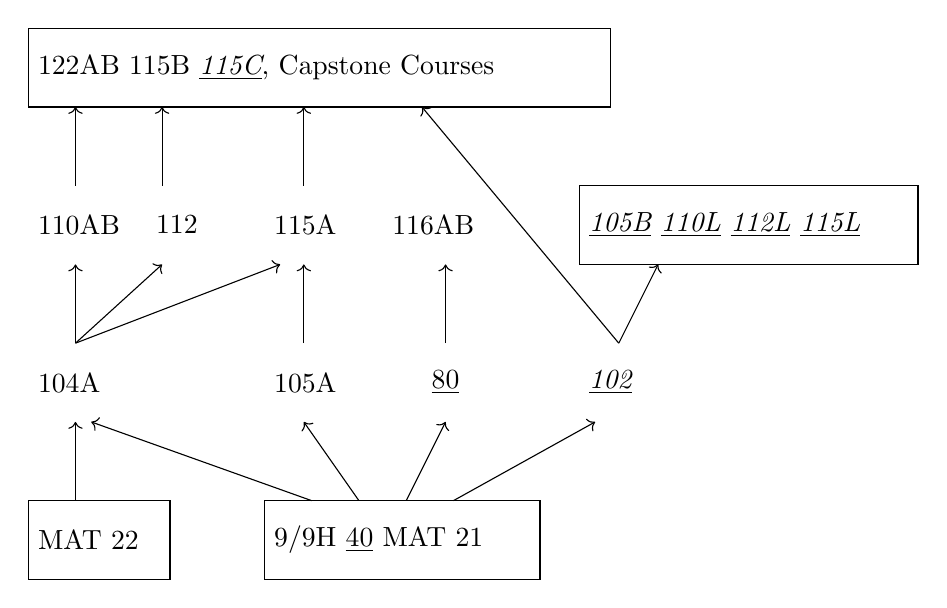
\begin{tikzpicture}

% 1st tier:
\node[right] at (0,0.5) {MAT 22};
\draw (0,0) coordinate(X) -- ++(0,1) -- ++(1.8,0) |- (X);

\node[right] at (3,0.5) {9/9H \underline{40} MAT 21};
\draw (3,0) coordinate(X) -- ++(0,1) -- ++(3.5,0) |- (X);



\draw[->] (0.6,1) --(0.6,2);
\draw[->] (3.6,1) --(0.8,2);
\draw[->] (4.2,1) --(3.5,2);
\draw[->] (4.8,1) --(5.3,2);
\draw[->] (5.4,1) --(7.2,2);
%\draw[->] (7.4,1) --(7.4,2);
%\draw[->] (7.2,1) --(5.5,2);


% 2nd tier:
\node[right] at (0,2.5) {104A};
%\draw (0,2) coordinate(X) -- ++(0,1.0) -- ++(1.2,0) |- (X);

\node[right] at (3,2.5) {105A};

\node[right] at (5,2.5) {\underline{80}};

\node[right] at (7,2.5) {\it \underline{102}};



\draw[->] (0.6,3) --(0.6,4);
\draw[->] (0.6,3) --(1.7,4);
\draw[->] (0.6,3) --(3.2,4);

\draw[->] (3.5,3) --(3.5,4);

\draw[->] (5.3,3) --(5.3,4);

\draw[->] (7.5,3) --(5,6);
\draw[->] (7.5,3) --(8.0,4);


% 3rd tier:
\node[right] at (0,4.5) {110AB};

\node[right] at (1.5,4.5) {112};

\node[right] at (3,4.5) {115A};

\node[right] at (4.5,4.5) {116AB};

\node[right] at (7,4.5) {\it \underline{105B} \underline{110L} \underline{112L} \underline{115L}};
\draw (7,4) coordinate(X) -- ++(0,1) -- ++(4.3,0) |- (X);

\draw[->] (0.6,5) --(0.6,6);
\draw[->] (1.7,5) --(1.7,6);
\draw[->] (3.5,5) --(3.5,6);


% top tier:
\node[right] at (0,6.5) {122AB 115B {\it \underline{115C}}, Capstone Courses};
\draw (0,6) coordinate(X) -- ++(0,1) -- ++(7.4,0) |- (X);


\end{tikzpicture}
\caption{\label{fig:prereqs} The prerequisite structure of physics and related math courses.  Courses within a box may have an internal prerequisite structure not shown.
For clarity, in some cases only the most advanced prerequisite are shown.  Prerequisites within a sequence (e.g. 112L has concurrent prerequisite with 112) are not shown.  All required courses are shown.  Underlines courses have a significantly computational component.  Italicized courses can be omitted from the requirements for Astrophysics or Applied Physics majors.}
\end{center}
\end{figure}

An overview of the prerequisite structure is shown in Fig.~\ref{fig:prereqs}.  
The graph reveals 104A as a major bottleneck in our program, as it requires the most advanced material from the first tier (MTH 22) but is required for most upper division classes, such as 110A and 115A.  The committee spend a great deal of time considering different ways to relieve or accommodate this bottleneck but in the end decided two offerings is the only effective way to achieve the goals of this proposal.  This stems from the fact that incoming transfer students must start on 104A immediately upon arrival in fall to complete the remaining upper division courses in two years, but sophomores finishing 9HD in the fall are not generally ready to take 104A until the spring.  

It appears from the graph that 102 is a bottleneck as well, but it is less severe.  It does not require MAT 22A so can be taken sooner than 104A, and it is only needed for top tier courses such 115C and the labs, which can be postponed until senior year.

The most notable changes are that:
\begin{itemize}
\item 80 adds 40 as a prerequisite.
\item 112 does not require 115A anymore, 104A and 9A-D must suffice instead.
\item 110A does not require 105A anymore. 
\item 105B and 115C require 102, which allows for computing to be integrated with these course. 
\end{itemize}
Some classes can be globally substituted as prerequisites, which we note here:
\begin{itemize}
\item Any ECS introductory programming course can replace 40.
\end{itemize}

\section{Discussion of Capstones and Electives}

Because 115A will be taught in the fall instead of spring, cap stone courses with 115A as a pre-requisite should start in the winter, with second quarter in spring.  We should take care to offer sufficient electives and capstones (without a 115A requirement) in spring.  We might want to consider a 3-credit upper division course dedicated to our arriving transfer students in the Fall, which will focus on consolidation and problem solving from the 9 series.  This could also be recommended for students that performed marginally in the 9 series.

\section{AB, Applied Physics Majors, and Astrophysics Specialization}

I'll add some discussion here:  we remove 102, 105B, 115C, 110L, 112L, and 115L.

\section{Study Abroad}

As a demonstration of the increased flexibility in the new program, I will add a plausible schedule for studying aboard in the junior year for students taking Honor's physics, which only requires them to find a 110AB equivalent while abroad.

\end{document}

\section{Detailed course listings - Preparatory Material}

For reference, the content in core required courses in the present catalog is included here:

\begin{itemize}

\item {\bf PHY 9A - Classical Physics (5)}
{\it Lecture—3 hours; laboratory—2.5 hours; discussion—1 hour. Prerequisite: Mathematics 21B. Introduction to general principles and analytical methods used in physics for physical science and engineering majors. Classical mechanics. Only 2 units of credit to students who have completed course 1A or 7B. Not open for credit to students who have completed course 9HA. GE credit: SciEng | SE. - III. (III.)}

\item {\bf PHY 9B - Classical Physics (5)}
{\it Lecture - 3 hours; laboratory - 2.5 hours; discussion - 1 hour. Prerequisite: course 9A [or 9HA], Mathematics 21C, 21D (may be taken concurrently). Continuation of course 9A. Fluid mechanics, thermodynamics, wave phenomena, optics. Only 2 units of credit to students who have completed course 7A. Not open for credit to students who have completed course 9HB, 9HC, or Engineering 105. - I. (I.)}

\item {\bf PHY 9C - Classical Physics (5)}
{\it Lecture - 3 hours; laboratory - 2.5 hours; discussion - 1 hour. Prerequisite; course 9B [or 9HC], Mathematics 21D, 22A (may be taken concurrently). Electricity and magnetism including circuits and Maxwell’s equations. Only 3 units of credit to students who have completed course 7C. Not open for credit to students who have completed course 9HD. GE credit: SciEng | SE. - II. (II.)}

\item {\bf PHY 9D - Modern Physics (4)}
{\it Lecture - 3 hours; discussion - 1.5 hours. Prerequisite: course 9C [or 9HD] and Mathematics 22A; Mathematics 22B recommended (may be taken concurrently). Introduction to physics concepts developed since 1900. Special relativity, quantum mechanics, atoms, molecules, condensed matter, nuclear and particle physics. Not open for credit to students who have completed course 9HB, 9HC, or 9HE. GE credit: SciEng | SE.- III. (III.)}

\item {\bf PHY 9HA - Honors Physics (5)}
{\it Lecture - 3 hours; discussion/laboratory - 4 hours. Prerequisite: Mathematics 21B (may be taken concurrently) or consent of instructor. Classical mechanics. Same material as course 9A in greater depth. For students in physical sciences, mathematics, and engineering. Only 2 units of credit to students who have completed course 7B. Not open for credit to students who have completed course 9A. GE credit: SciEng | SE. - I. (I.)}

\item {\bf 9HB - Honors Physics (5)}
{\it Lecture - 3 hours; discussion/laboratory - 4 hours. Prerequisite: Physics 9HA or 9A, Mathematics 21C (may be taken concurrently). Special relativity, thermal physics. Continuation of course 9HA. Only 2 units of credit to students who have completed course 7A. Not open for credit to students who have completed course 9B or 9D. GE credit: SciEng | SE. - II. (II.)}

\item {\bf 9HC - Honors Physics (5)}
{\it Lecture - 3 hours; discussion/laboratory - 4 hours. Prerequisite: course 9HB and Mathematics 21D (may be taken concurrently). Waves, sound, optics, quantum physics. Continuation of Physics 9HB. Only 2 units of credit to students who have completed course 7C. Not open for credit to students who have completed course 9B or 9D. GE credit: SciEng | SE.- III. (III.)
Recent Syllabi and More Complete Descriptions}

\item {\bf 9HD - Honors Physics (5)}
{\it Lecture - 3 hours; discussion/laboratory - 4 hours. Prerequisite: course 9HC and Mathematics 21D. Electricity and magnetism. Continuation of Physics 9HC. Not open for credit to students who have completed course 9C. GE credit: SciEng | SE. - I. (I.)}

\item {\bf 9HE - Honors Physics (5)}
{\it Lecture - 3 hours; discussion/laboratory - 4 hours. Prerequisite: course 9HD and Mathematics 22B (may be taken concurrently). Application of quantum mechanics. Not open for credit to students who have completed course 9D. GE credit: SciEng | SE. - II. (II.)}

\item {\bf PHY 40 — Introduction to Physics Computation (4)}
{\it Lecture—2 hour(s); Laboratory—4 hour(s). Introduction to programming using C++ with examples from computational physics. Introduction to modern tools used for scientific analysis, including Scientific computing with Python. GE credit: SE. Effective: 2018 Summer Session 2.}

\item {\bf PHY 80 — Experimental Techniques (4)}
{\it Lecture—2 hour(s); Laboratory—5 hour(s). Prerequisite(s): PHY 009D or PHY 009HD. Open to Physics and Applied Physics majors only. Experimental techniques. Design of circuits. Data analysis, sources of noise, statistical and systematic uncertainties. Light sources, detection, and measurement in basic optical systems. Effective: 2017 Fall Quarter.}

\end{itemize}

\section{Detailed course listings - Core Subject Matter}

\begin{itemize}
\item {\bf PHY 104A - Introductory Methods of Mathematical Physics}
{\it Lecture - 3 hours; extensive problem solving. Prerequisite: courses 9B, 9C, 9D [or 9HB, 9HC, 9HD] and Mathematics 21D, 22A, and 22B with grade C- or better or consent of instructor. Introduction to the mathematics used in upper-division physics courses, including applications of vector spaces, Fourier analysis, partial differential equations. - I. (I.)}

Recently taught by Scalettar and Luty.  Luty teaches this as a boot camp for upper division courses:  vectors, expansion in small parameters, and PDEs.  All topics which are in principle should have been seen before, but students clearly need practice with problems.

\item {\bf PHY 105A - Analytical Mechanics}
{\it Lecture - 3 hours; extensive problem solving. Prerequisite: courses 9B, 9C, 9D [or 9HB, 9HC, 9HD] and Mathematics 21D, 22A, and 22B passed with grade C– or better; or consent of department; course 104A and 105A passed with a grade C– or better or consent of department required for 105B. Principles and applications of Newtonian mechanics; introduction to Lagrange’s and Hamilton’s equations. - I-II. (I-II.)}

Recently taught by Calderon, Cebra, Svoboda, and Conway.  Covers Morin 1-5.  This course is heavy on problem solving.  Morin focuses more on challenging problems, and less on mathematical formalism (e.g. leaves out Hamiltonian)
Not all instructors reach 5 in first quarter.

\item {\bf PHY 105B - Analytical Mechanics}
{\it Lecture - 3 hours; extensive problem solving. Prerequisite: courses 9B, 9C, 9D [or 9HB, 9HC, 9HD] and Mathematics 21D, 22A, and 22B passed with grade C– or better; or consent of department; course 104A and 105A passed with a grade C– or better or consent of department required for 105B. Principles and applications of Newtonian mechanics; introduction to Lagrange’s and Hamilton’s equations. - I-II. (I-II.)}

Recently taught by Pickett, Conway.  Covers Morin 6-11.  Picket supplement chapter 5 with supplemental material for Hamiltonian.

\item {\bf PHY 110A - Electricity and Magnetism}
{\it Lecture - 3 hours; extensive problem solving. Prerequisite: courses 9B, 9C, 9D [or 9HB, 9HC, 9HD] and Mathematics 21D, 22A, and 22B passed with grade C– or better, or consent of department; prerequisite for 110B is courses 110A and 104A passed with a grade of C– or better or consent of department; prerequisite for course 110C is courses 110B and 104B passed with a grade of C– or better, or consent of department. Theory of electrostatics, electromagnetism, Maxwell’s equations, electromagnetic waves. - II-III-I. (II-III-I.)}

Recently taught by Da Silva Neto and Yu.  Covers Griffiths 1-4.  Yu extends to include complex analysis of La Place's equation.  Includes a recap of vector calculus, but Da Silva Neto reports a benefit from 104A  (Math Methods.)

\item {\bf PHY 110B - Electricity and Magnetism}
{\it Lecture - 3 hours; extensive problem solving. Prerequisite: courses 9B, 9C, 9D [or 9HB, 9HC, 9HD] and Mathematics 21D, 22A, and 22B passed with grade C– or better, or consent of department; prerequisite for 110B is courses 110A and 104A passed with a grade of C– or better or consent of department; prerequisite for course 110C is courses 110B and 104B passed with a grade of C– or better, or consent of department. Theory of electrostatics, electromagnetism, Maxwell’s equations, electromagnetic waves. - II-III-I. (II-III-I.)}

Recently taught by Yu.  Griffiths 5-9.  Rapid pace for subject matter, so problem solving is left mainly for homework.  No breathing room for computational physics.

\item {\bf PHY 110C - Electricity and Magnetism}
{\it Lecture - 3 hours; extensive problem solving. Prerequisite: courses 9B, 9C, 9D [or 9HB, 9HC, 9HD] and Mathematics 21D, 22A, and 22B passed with grade C– or better, or consent of department; prerequisite for 110B is courses 110A and 104A passed with a grade of C– or better or consent of department; prerequisite for course 110C is courses 110B and 104B passed with a grade of C– or better, or consent of department. Theory of electrostatics, electromagnetism, Maxwell’s equations, electromagnetic waves. - II-III-I. (II-III-I.)}

Recently taught by Yu and Luty.  Rest of Griffiths.   Potentials (including vector potential), radiation in matter, special relativity.

\item {\bf PHY 112 - Thermodynamics and Statistical Mechanics}
{\it Lecture - 3 hours; extensive problem solving. Prerequisite: course 115A or the equivalent. Introduction to classical and quantum statistical mechanics and their connections with thermodynamics. The theory is developed for the ideal gas model and simple magnetic models and then extended to studies of solids, quantum fluids, and chemical equilibria. - I. (I.)}

Recently taught by Singh, Da Silva Neto.  Based on Shroeder.  
Fast review of 1 (Thermodynamics), full coverage of 2 and 3 (Entropy/Temperature starting from quantum systems up to ideal gas) skip 4 (Heat engines), Free energy part of 5, full coverage of 6+7 (Boltzman and Quantum statistics).

\item {\bf PHY 115A - Foundation of Quantum Mechanics}
{\it Lecture - 3 hours; extensive problem solving. Prerequisite: courses 104A and 105A with grade C- of better, or consent of instructor. Introduction to the methods of quantum mechanics with applications to atomic, molecular, solid state, nuclear and elementary particle physics. - III. (III.)} 

Recently taught by Fong,Curro.  Townsend for undergraduate version of Sakurai's spin-first approach.  Chapters 1-5, sometimes 6.

\item {\bf PHY 115B - Applications of Quantum Mechanics}
{\it Lecture - 3 hours; extensive problem solving. Prerequisite: course 115A passed with a grade of C– of better, or consent of department. Angular momentum and spin; hydrogen atom and atomic spectra; perturbation theory; scattering theory. - I. (I.)}

Recently taught by Curro.  Townsend 6,7, skip 8 (path integrals), then 9-10.
Leaves off perturbation theory, identical particles, scattering.

\end{itemize}
\end{document}
